\section{类别错误归因}

\subsection{总体混淆结构}

采用 R(2+1)D-18 在种子 0 的官方测试预测生成 $101\times101$ 混淆矩阵，如图
\ref{fig:confusion} 所示。矩阵按真实类别归一化，对角线越亮表示召回越高。

\begin{figure}[H]
  \centering
  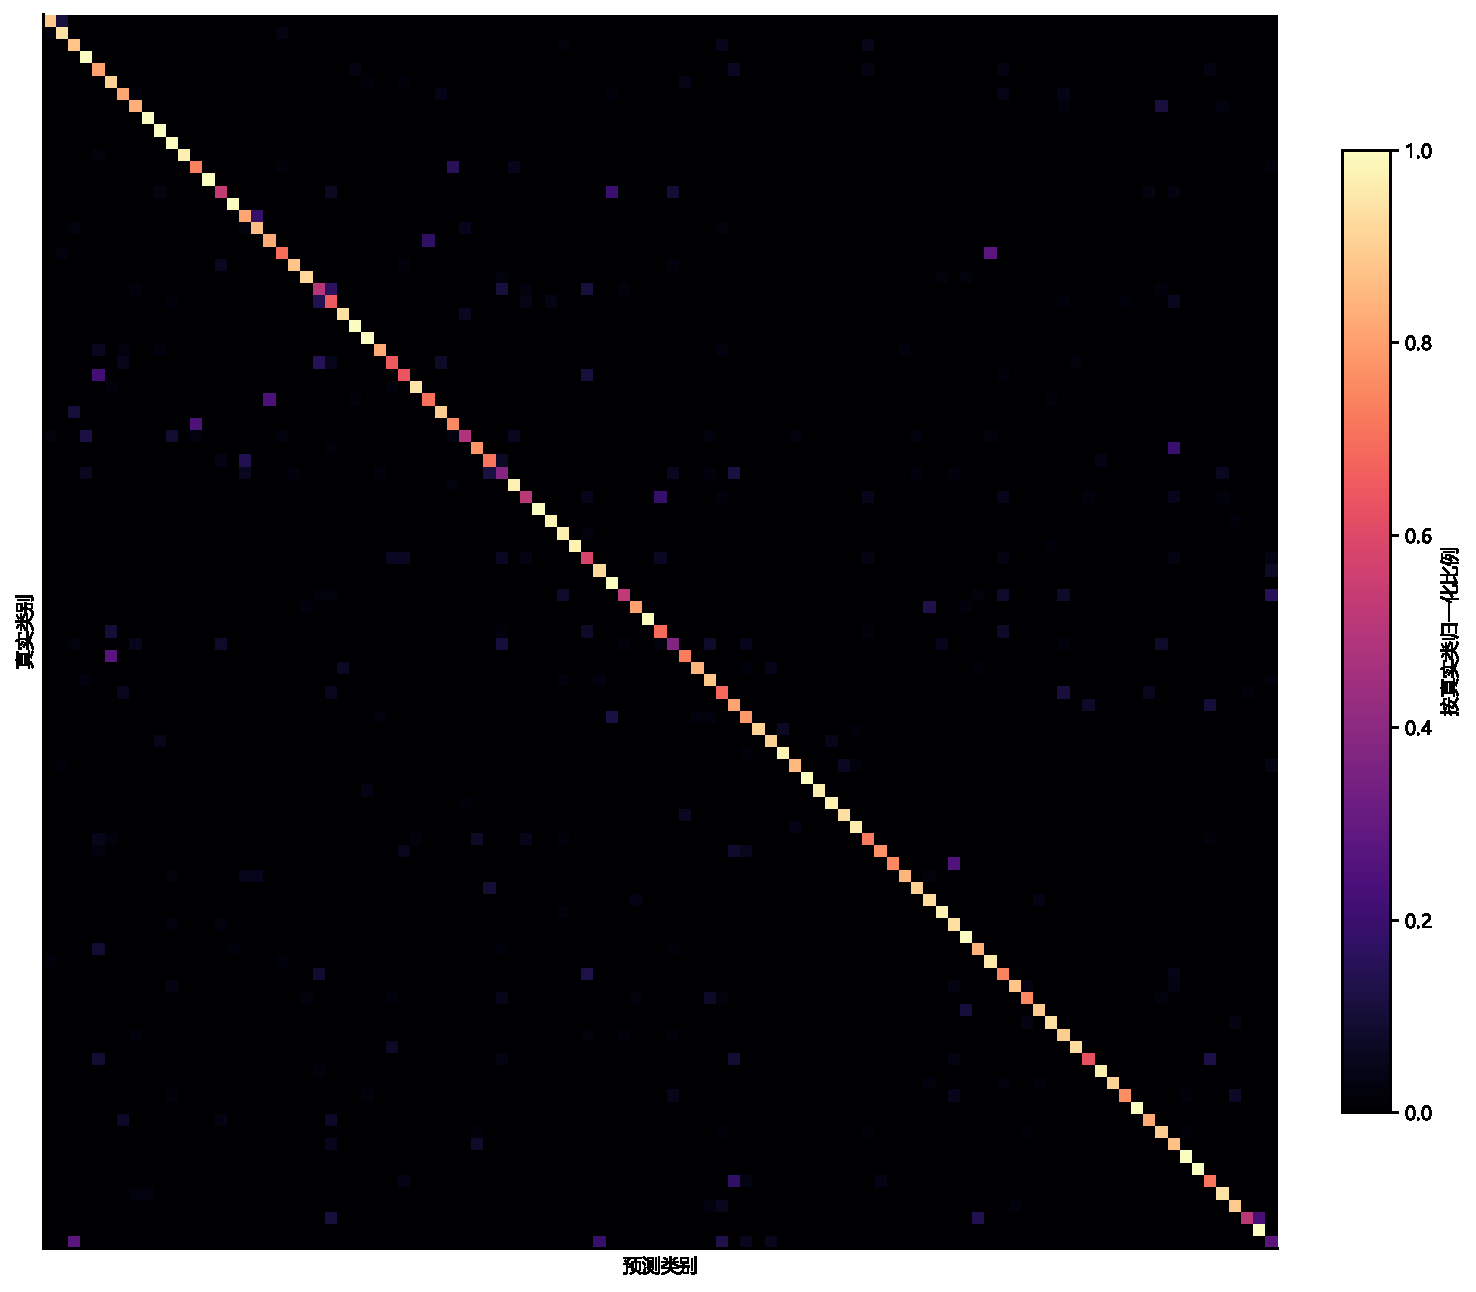
\includegraphics[width=0.76\textwidth]{../../results/feature_pipeline/main_20261125_193324/error_analysis/r2plus1d18/confusion_matrix.pdf}
  \caption{R(2+1)D-18 的 101 类归一化混淆矩阵}
  \label{fig:confusion}
\end{figure}

主要非对角混淆对包括：
\begin{itemize}
  \item BrushingTeeth 与 ShavingBeard，均包含面部近景和重复手部动作；
  \item YoYo 与 Archery、JugglingBalls，手势和细长物体轨迹相似；
  \item BoxingPunchingBag 与 BoxingSpeedBag，空间场景几乎一致；
  \item FrontCrawl 与 BreastStroke，水下场景相似但周期动作不同；
  \item CricketShot 与 CricketBowling，共享运动场地、器材和人物尺度。
\end{itemize}

这些错误说明，当视频背景高度相似、动作差异集中在短时阶段时，全局池化表示仍会
压缩掉关键时间线索。

\subsection{分类别表现}

最低召回的五个类别为 YoYo、Lunges、HandstandWalking、Hammering 和
CricketBowling，召回率分别为 27.78\%、37.84\%、38.24\%、48.48\% 和 50.00\%。
这些类别的共同特征是细粒度人体姿态、重复周期动作或多个相似动作阶段。

图~\ref{fig:group} 将 101 类按语义分为人际交互、人体动作、物体交互、演奏乐器
和体育运动五组。该分组用于解释错误结构，不替代官方 101 类标签。

\begin{figure}[H]
  \centering
  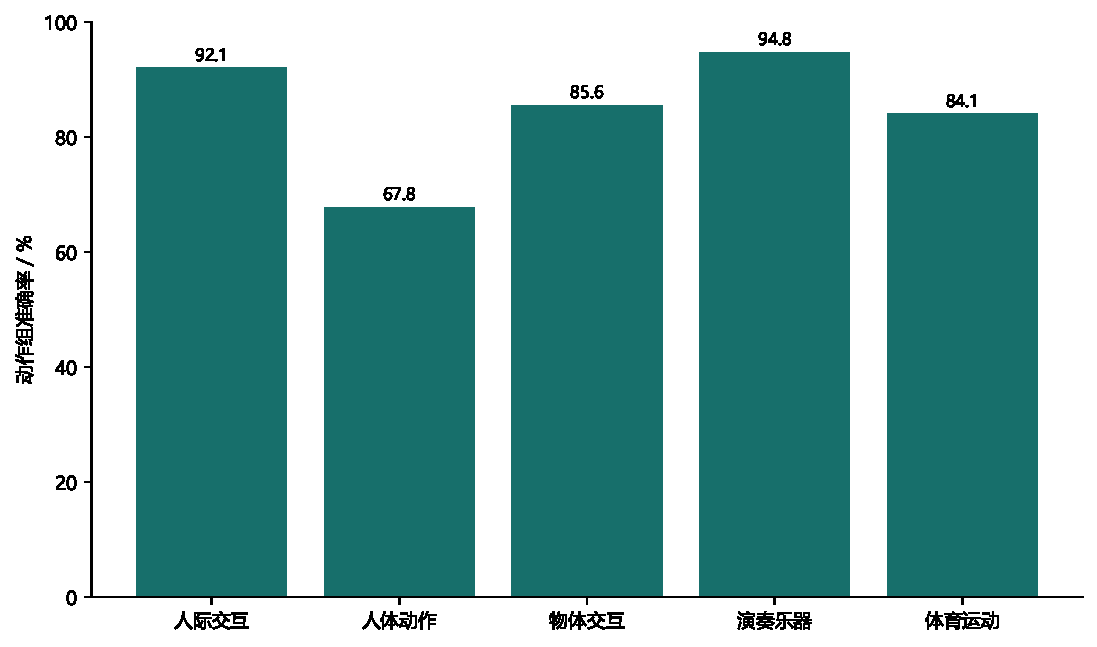
\includegraphics[width=0.72\textwidth]{../../results/feature_pipeline/main_20261125_193324/error_analysis/r2plus1d18/action_group_accuracy.pdf}
  \caption{动作语义组的测试准确率}
  \label{fig:group}
\end{figure}

人体动作组只有 67.78\%，明显低于演奏乐器的 94.76\% 和人际交互的 92.05\%。
乐器演奏通常具有稳定的物体和场景，动作关键阶段也较突出。人体动作组则更容易
受到体态比例、拍摄角度和阶段选取影响。

\subsection{代表性失败模式}

第一类是“静态外观相似”。R3D-18 与 TSN 都可能把 BrushingTeeth 判为
ShavingBeard，因为两者同时出现人脸近景、手部和重复动作。此时全局空间上下文
占据主导，8 帧中若未采到牙刷或剃刀的关键细节，时间聚合也无法纠正。

第二类是“时间阶段缺失”。连续稠密采样在投掷、跳跃和水泳类动作上更易失败。
均匀采样覆盖全视频，因此总体准确率更高。

第三类是“细粒度周期运动”。YoYo、JumpRope、JugglingBalls 与
PlayingDhol 都有周期性手部运动，但它们对应的物体和运动轨迹不同。当前二维
逐帧特征主要依赖物体外观，无法稳定恢复运动方向。

上述失败模式意味着下一步应优先增加空间分辨率或引入局部时序模块，而不是继续
增加低分辨率帧数。更细粒度的光流或轨迹特征可作为后续扩展。
